\documentclass[a4paper,10pt]{article}
\usepackage[utf8]{inputenc}
\usepackage{graphicx}
\graphicspath{ {./code/} }


\title{\textbf{GAMA and Agents} \\ 
\textbf{Assignment I}}

\author{Emil Ståhl and Peyman Peirovifar}

\begin{document}

\maketitle
\textbf
{\\1. Introduction\\\\}
This report covers the implementation of a multi agent-based festival simulation written in the modeling language GAMA. The continuously running simulation consists of three types of agents that are guests, store or information center. The guests wander around the festival area until they either become hungry or thirsty, the guests then goes to a known location where the information center resides. At the information center the guests asks for directions to where to find the store for food or drinks. After the guest has visited the store they go back to wandering around the festival until they need to repeat the steps. The goal of this work is to get an introduction to the GAMA platform and working with agents as well as obtain experience of the syntax and how basic simulations work along with basic principles for distributed intelligent agents.


\maketitle
\textbf
{\\2. The program and its purposes\\\\}
The program consists of three types of agents/species (similar to classes in objective oriented programming). These agents are as previously stated guests, stores or information center. 

\maketitle
\textbf
{\\3. Implementation\\\\}
A GAMA model contains a unique global section that defines the global species. Here we initialize some variables and points for later use. After the initialization is done the different species /agents are spawned at a specified location with the \texttt{create} keyword. The location of the different stores and pubs are also given to the information center so that agents can request their location from the information center. \\\\The next step is to define the different species/agents and their behaviors and appearance. Information center is defined with its required location of the stores and pubs as well as given an aspect that specifies that it should be displayed as a red cylinder at the location that was given at initialization. Aspects for the species \texttt{WC, Pub} and \texttt{Restaurant} are given in a similar manner.
\\\\Next up is the \texttt{Guest} species which is given a few reflexes that defines its behavior. Firstly, a bunch of variables and points are declared that are going to be used in the reflexes. The aspect is defined as a sphere of the color given in the declaration above. The \texttt{Guest} species/agent first reflex is \texttt{goToInfo}, this reflex is performed when one of the variables \texttt{WC, thirst} or \texttt{hunger} drops below the value of zero. A boolean flag \texttt{informed} is used to check if the agent has been given the location or not, if false the reflex if performed. \\\\The guest knows the location of the information center. The reflex consists of several if clauses,  the outermost if-statement checks if the guest has arrived at the information center, when this becomes true the guest checks if the queue to the information center is empty, if so the reflex enters the correct if-statement depending on which variable that caused the reflex to trigger. The if-statements for this works in a similar manner which is that it utilizes the ask keyword to specify what location it want to know. The information center gives this point to the guest which saves it in its \texttt{targetpoint} variable. After this, the boolean flag informed is set to true which triggers the next reflex \texttt{fromInformationCentre} to be triggered. \\\\The reflex \texttt{fromInformationCentre} is performed once the guest has got the desired location and the flag is set to true. First thing is to check which location to go to, this is done with a simple if-statement. When \texttt{targetpoint} is set, the guest goes to the location by using the goto keyword. When arrived it waits for its turn and then executes the correct if-statement. Inside each if-statement, the value of the variable is reset to an arbitrary value between 100 and 300. The queue is also decremented. Lastly, the informed flag is reset to false and the guest is given a new random point to go dance at. \\\\When a guest \texttt{targetpoint} is not specified and its hunger and thirst variables doesn’t equal zero it executes the reflex \texttt{fromCheckPoint}. This reflex is responsible for resetting \texttt{targetpoint} to nil, decrement the variables of hunger and thirst and make the agent wander dance around the festival area. The last reflex is \texttt{beIdle} which executes when the \texttt{targetpoint} has been set to nil by \texttt{fromCheckPoint}. When all species and their reflexes has been defined we just need to define an experiment for the model to run in. We define an experiment \texttt{gui} and just state that all species should be displayed.
\clearpage
\maketitle
\textbf
{\\\\4. Results\\\\}
Shown below is part of the message log and a snapshot of the simulation running. 
\begin{verbatim}
Guest5says: I am thirsty.
Guest5says: Thanks, I got it!
Guest3says:I am relieved!
Guest28says:I am relieved!
Guest16says: I am thirsty.
Guest16says: Thanks, I got it!
Guest42says: I need to go bathroom.
Guest42says: Thanks, I got it!
Guest15says: I need to go bathroom.
Guest15says: Thanks, I got it!
Guest41says:I am relieved!
Guest13says: I need to go bathroom.
Guest13says: Thanks, I got it!
Guest34says:I am relieved!
Guest43says:Nice Let's go back to dancing
\end{verbatim}

\begin{center}{}
\centering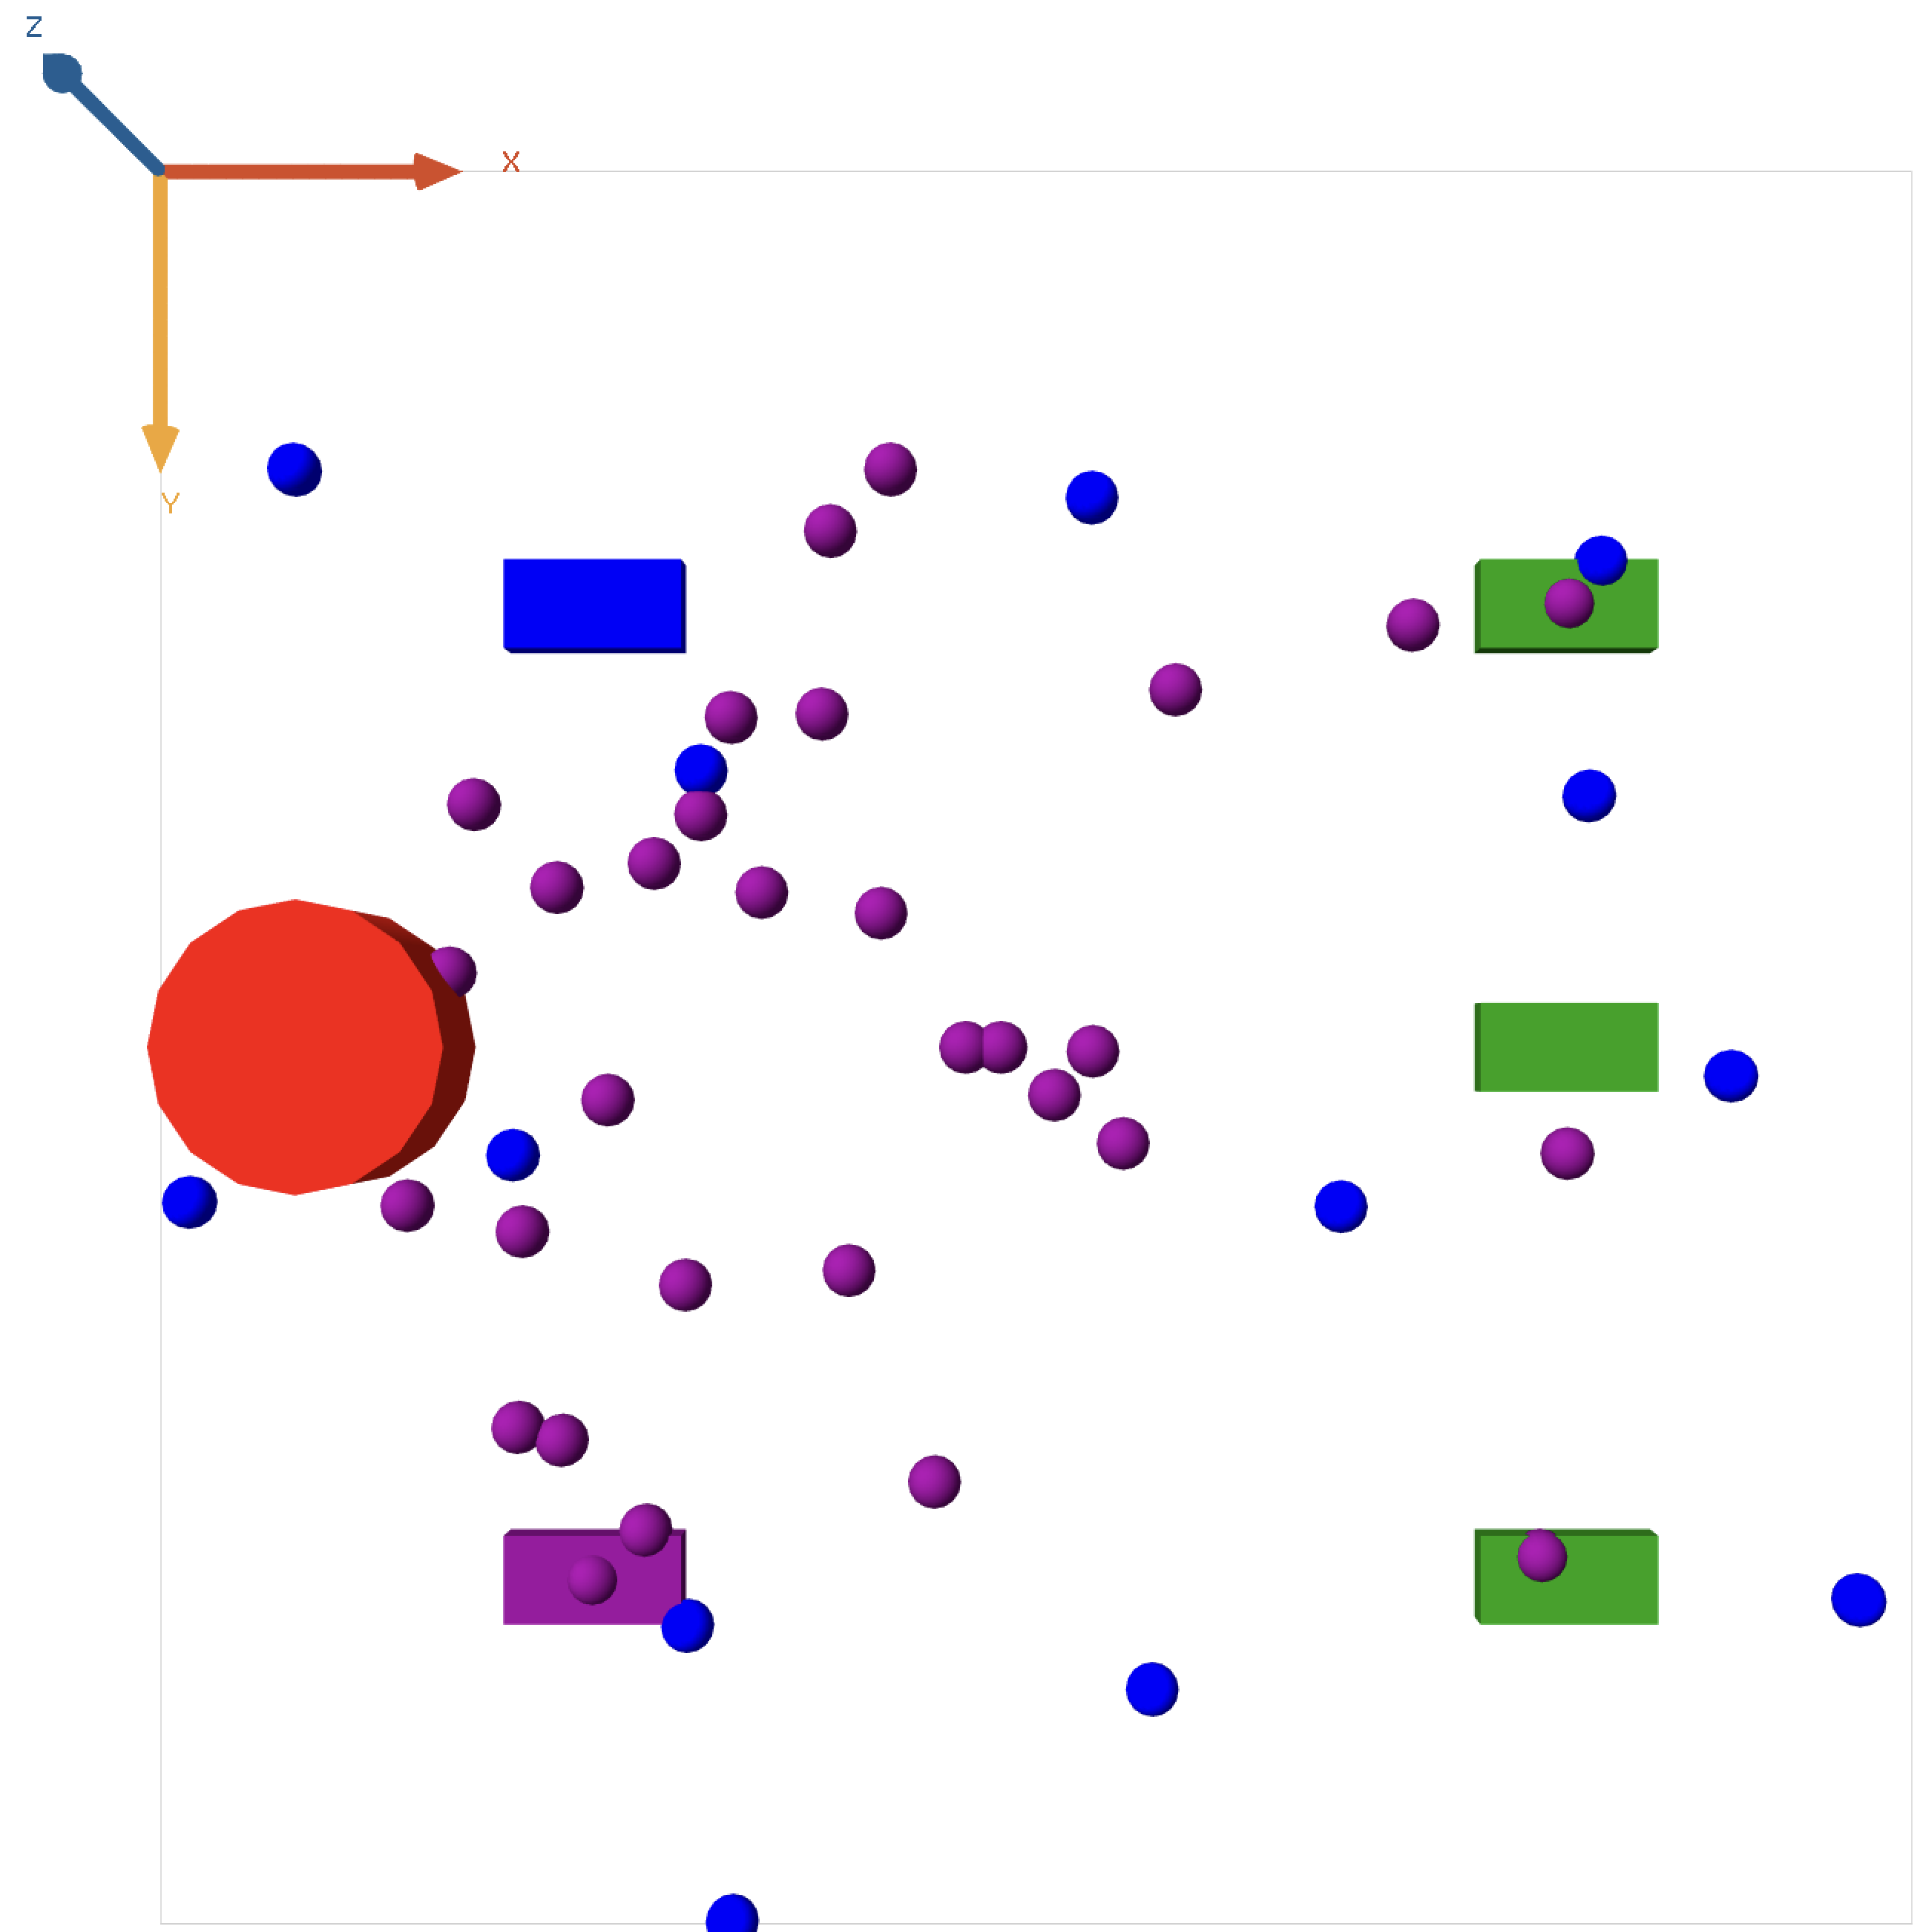
\includegraphics[scale=0.1]{Simulation.png}\par
\end{center}

\clearpage
\maketitle
\textbf
{\\\\5. Conclusions\\\\}
This work an introduction to the GAMA platform, its syntax and the fundamentals of working with agents. The most challenging part was to understand how the GAMA platform and language worked, it offers a quite different way of structuring a program. 

\end{document}
